% Please include the author-supplied PDF unchanged and retain the existing label.
% Source attachment: de757cd7-77d6-4058-9436-f652c5046293/fig2_votes.pdf.
% SHA-256: a3f79400cdf48f23196f4c553b87d2c0fa6c1faa968b9c86b879c59ebb532041.
% The previous TikZ version remains available but is not compiled here.
\begin{figure}[H]
\centering
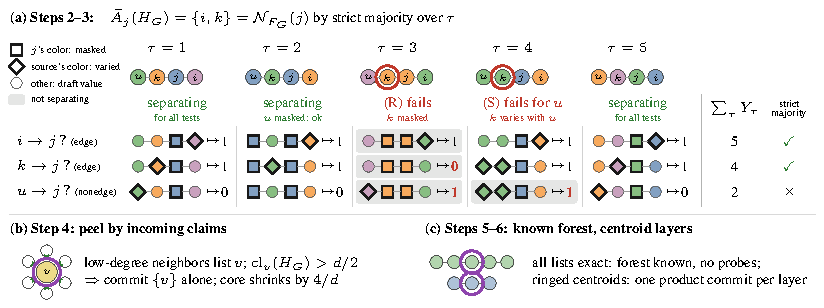
\includegraphics[width=\linewidth]{figures/algorithm_examples_2026-09-18/fig2_votes_2026-09-26_002617_JST.pdf}
\caption{\textcolor{red}{Shared tests and majority recovery.
(a) Each cell represents all bank/tail columns; each readout color has one
chunk. Equal-color pairs (no diamond) get vote $0$ without probing.
Grey: nonseparation; red: illustrative errors.
(b) Singleton peels contract the core per phase.
(c) One centroid per component forms a terminal batch.}}
\label{fig:algorithm-overview-20260918}
\end{figure}
